\subsection{1.2. Khảo sát bài toán}

\subsubsection{1.2.1. Khảo sát các biểu mẫu và các tài liệu nghiệp vụ thực tế}
Nhóm thực hiện đã tiến hành khảo sát và thu thập 03 nhóm biểu mẫu, tài liệu nghiệp vụ thực tế đang được sử dụng phổ biến trong hoạt động học tập và giảng dạy tại Khoa Công nghệ Thông tin, Trường Đại học Sư phạm TPHCM:

\paragraph{a) Kế hoạch bài dạy theo chuẩn Công văn 5512/BGDĐT-GDTrH}
\begin{figure}[H]
\centering
\IfFileExists{chuong1/images/hinh_1_1a_khbd_5512.jpg}{%
    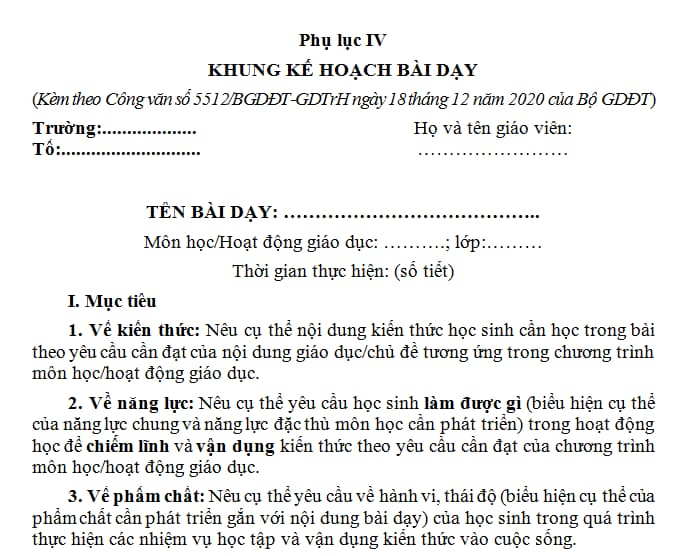
\includegraphics[width=0.88\textwidth]{chuong1/images/hinh_1_1a_khbd_5512.jpg}%
}{%
    \fbox{\parbox{0.88\textwidth}{\centering \vspace{2cm}\textbf{[Hình 1.1a: Khung Kế hoạch bài dạy chuẩn Công văn 5512 của Bộ GD\&ĐT]}\vspace{2cm}}}%
}
\caption{Khung Kế hoạch bài dạy chuẩn Công văn 5512 của Bộ GD\&ĐT}
\label{fig:khbd_5512}
\end{figure}

Đây là biểu mẫu nghiệp vụ sư phạm cốt lõi của sinh viên ngành Sư phạm Tin học. Một bản Kế hoạch bài dạy chuẩn theo hướng dẫn của Bộ Giáo dục và Đào tạo có cấu trúc thống nhất bao gồm: Mục tiêu dạy học (về kiến thức, năng lực và phẩm chất); Thiết bị dạy học và học liệu; cùng Tiến trình dạy học gồm 4 hoạt động bắt buộc:
\begin{itemize}[leftmargin=*,noitemsep]
    \item \textbf{Hoạt động Khởi động:} Giúp học sinh xác định được mâu thuẫn nhận thức hoặc nhiệm vụ cần thực hiện.
    \item \textbf{Hoạt động Hình thành kiến thức mới:} Học sinh tiếp nhận tri thức mới thông qua hướng dẫn và hoạt động học tập cụ thể.
    \item \textbf{Hoạt động Luyện tập:} Học sinh làm bài tập để củng cố và khắc sâu kiến thức.
    \item \textbf{Hoạt động Vận dụng:} Vận dụng kiến thức, kỹ năng Tin học đã học để giải quyết bài toán thực tế đời sống.
\end{itemize}
Cấu trúc nghiệp vụ này được hệ thống 5Share sử dụng làm tiêu chuẩn đánh giá chất lượng tài liệu giáo án khi kiểm duyệt và thiết lập bộ thuộc tính lọc.

\paragraph{b) Đề thi kết thúc học phần}
Nhóm tiến hành thu thập và khảo sát các đề thi học phần các môn chuyên ngành như Cơ sở dữ liệu, Kiến trúc máy tính,... Đặc thù của tài liệu này đòi hỏi thông tin chính xác về học kỳ, năm học, thời lượng làm bài.

\begin{figure}[H]
\centering
\IfFileExists{chuong1/images/hinh_1_1b_de_thi_mmt.jpg}{%
    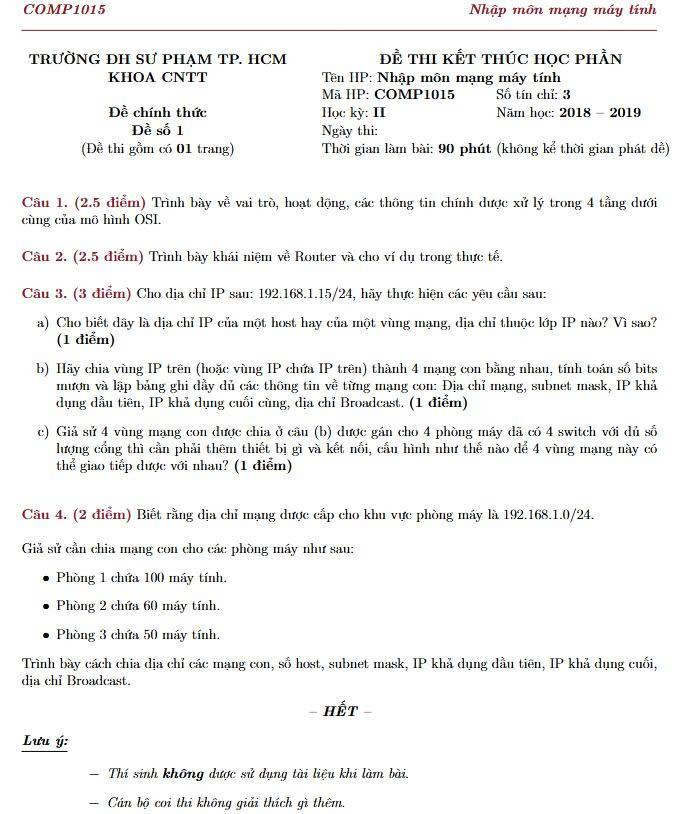
\includegraphics[width=0.88\textwidth]{chuong1/images/hinh_1_1b_de_thi_mmt.jpg}%
}{%
    \fbox{\parbox{0.88\textwidth}{\centering \vspace{2cm}\textbf{[Hình 1.1b: Đề thi kết thúc học phần môn Mạng máy tính năm học 2018-2019 (khoa CNTT, trường Đại học Sư phạm TPHCM)]}\vspace{2cm}}}%
}
\caption{Đề thi kết thúc học phần môn Mạng máy tính năm học 2018-2019 (khoa CNTT, trường Đại học Sư phạm TPHCM)}
\label{fig:de_thi_mmt}
\end{figure}

\paragraph{c) Bài giảng điện tử và đề cương học phần chuyên ngành}
Bao gồm các slide bài giảng lý thuyết, tài liệu hướng dẫn thực hành hoặc đề cương chi tiết học phần. Đặc điểm của nhóm học liệu này là tính trực quan, yêu cầu hiển thị nhanh trên trình duyệt để sinh viên dễ dàng tra cứu đề cương ôn tập.

\begin{figure}[H]
\centering
\IfFileExists{chuong1/images/hinh_1_1c_slide_ptct.png}{%
    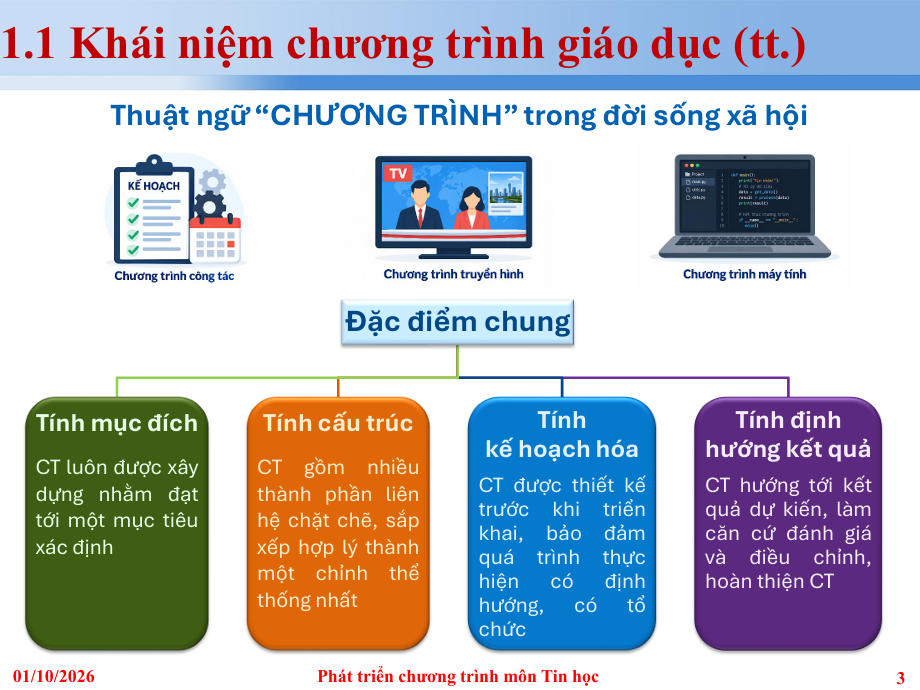
\includegraphics[width=0.88\textwidth]{chuong1/images/hinh_1_1c_slide_ptct.png}%
}{%
    \fbox{\parbox{0.88\textwidth}{\centering \vspace{2cm}\textbf{[Hình 1.1c: Slide bài giảng điện tử môn PTCT môn Tin học của Cô Nguyễn Trần Phi Phượng (trên MS Teams)]}\vspace{2cm}}}%
}
\caption{Slide bài giảng điện tử môn PTCT môn Tin học của Cô Nguyễn Trần Phi Phượng (trên MS Teams)}
\label{fig:slide_ptct}
\end{figure}

\subsubsection{1.2.2. Khảo sát người dùng bằng bảng câu hỏi}
Nhóm thực hiện đã triển khai phiếu khảo sát trực tuyến qua Google Forms và thu thập ý kiến đóng góp từ 17 sinh viên năm 3 ngành Sư phạm Tin học thuộc Trường Đại học Sư phạm TP.HCM. Kết quả khảo sát định lượng được thống kê chi tiết tại Hình 1.2:

\begin{figure}[H]
\centering
\IfFileExists{chuong1/images/hinh_1_2_khao_sat.png}{%
    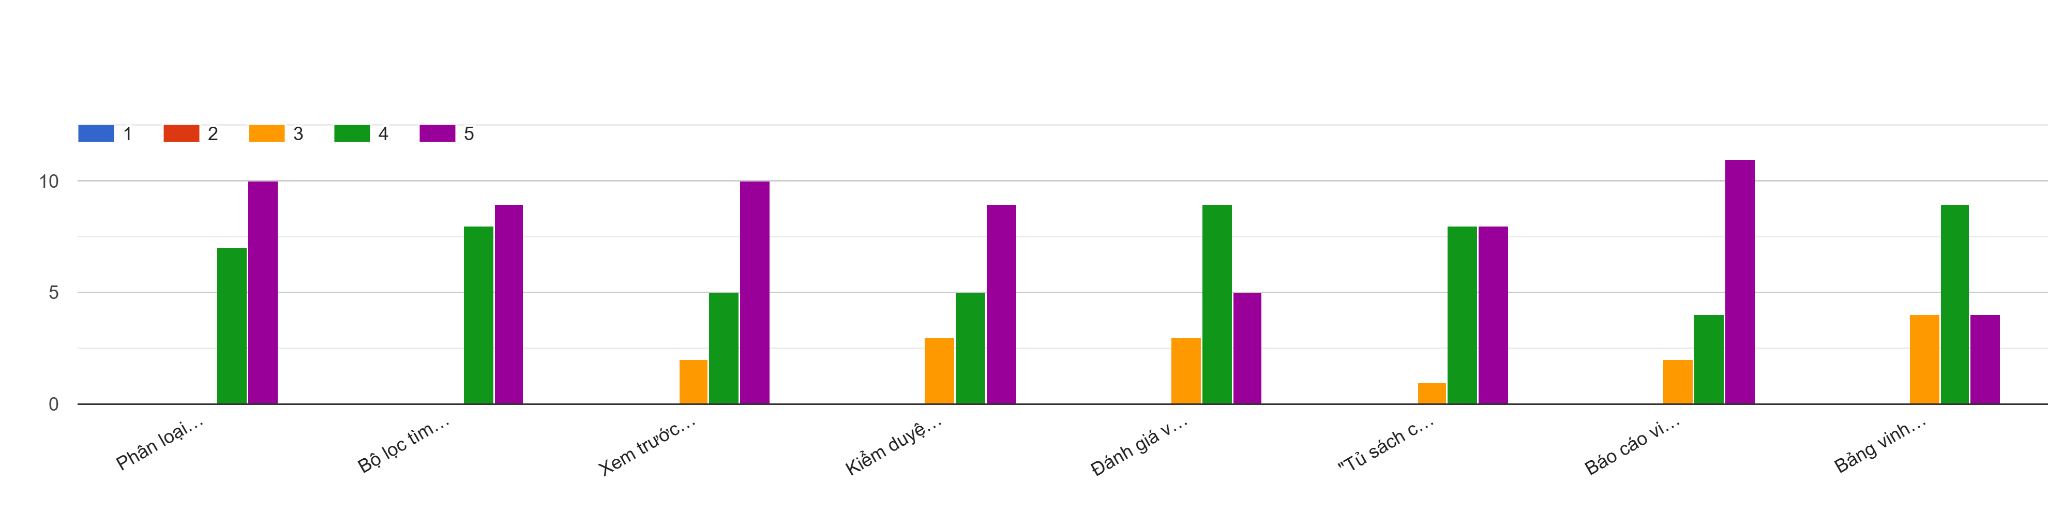
\includegraphics[width=0.92\textwidth]{chuong1/images/hinh_1_2_khao_sat.png}%
}{%
    \fbox{\parbox{0.92\textwidth}{\centering \vspace{2.5cm}\textbf{[Hình 1.2: Đánh giá của sinh viên về mức độ cần thiết của các tính năng trên hệ thống 5Share]}\vspace{2.5cm}}}%
}
\caption{Đánh giá của sinh viên về mức độ cần thiết của các tính năng trên hệ thống 5Share}
\label{fig:khao_sat_tinh_nang}
\end{figure}

Kết quả khảo sát tại Hình 1.2 phản ánh sự đồng thuận rất cao của sinh viên ngành Sư phạm Tin học đối với 8 nhóm tính năng được đề xuất cho hệ thống 5Share, trong đó phần lớn ý kiến đánh giá đều tập trung ở thang điểm 4 (Khá cần thiết) và thang điểm 5 (Rất cần thiết). Cụ thể:
\begin{itemize}[leftmargin=*,noitemsep]
    \item \textbf{Kiểm soát chất lượng học thuật:} phần lớn sinh viên tham gia khảo sát đánh giá tính năng ``Kiểm duyệt chất lượng trước khi đăng'' và ``Báo cáo vi phạm nội dung'' là thực sự cấp thiết. Thực tế khảo sát cho thấy sinh viên thường xuyên gặp rủi ro trước các nguồn tài liệu sai chuẩn hoặc trôi nổi trên mạng xã hội, do đó việc thiết lập hàng rào kiểm duyệt chuyên môn là yếu tố cốt lõi tạo nên giá trị và độ tin cậy của kho học liệu.
    \item \textbf{Tra cứu và trải nghiệm học liệu:} Tính năng ``Xem trước nội dung trực tiếp'' và ``Bộ lọc tìm kiếm thông minh'' được lượng sinh viên coi là cần thiết chiếm hơn 80\%. Sinh viên có nhu cầu đọc thử nhanh các trang đầu của tài liệu ngay trên trình duyệt để đánh giá độ phù hợp trước khi quyết định tải về máy, giúp tiết kiệm thời gian tra cứu và tối ưu dung lượng lưu trữ thiết bị.
    \item \textbf{Tương tác và tạo động lực cộng đồng:} Các tính năng ``Đánh giá và bình luận'', ``Tủ tài liệu cá nhân'' cũng được xếp loại mức độ là cần thiết vì bản thân sinh viên cũng cần có một không gian riêng để lưu trữ và một nơi để trao đổi về các tài liệu; ``Bảng vinh danh'' cũng tương tự như vậy, nhưng một phần sinh viên trung lập xem nó chỉ là tính năng phụ đi kèm. Đây là căn cứ thực tiễn quan trọng để hệ thống xem xét thiết kế cơ chế tích điểm cống hiến, vừa ghi nhận bản quyền tác giả, vừa thúc đẩy tinh thần chia sẻ học liệu tích cực trong cộng đồng sinh viên sư phạm.
\end{itemize}

\subsubsection{1.2.3. Khảo sát chuyên sâu thông qua phỏng vấn giả định}
Để tiếp cận sâu sắc góc nhìn chuyên môn của người trực tiếp tham gia giảng dạy và hướng dẫn chuyên môn, nhóm đã thực hiện phỏng vấn giả định chuyên sâu thông qua kỹ thuật đóng vai. Người phỏng vấn là sinh viên Nguyễn Trần Đăng Khoa và người được phỏng vấn là anh Huỳnh Anh Tuấn (cựu sinh viên ngành Sư phạm Tin học, hiện là Trợ giảng học phần Phương pháp dạy học môn Tin học).

\noindent \textbf{Nội dung tóm tắt biên bản phỏng vấn chuyên sâu:}
\begin{itemize}[leftmargin=*,noitemsep]
    \item \textbf{Khó khăn trong thực tế rèn nghề sư phạm:} Về thực trạng sinh viên chuẩn bị Kế hoạch bài dạy hiện nay, người được phỏng vấn nhận định sinh viên các khóa mới thường gặp khó khăn trong việc nắm vững cấu trúc 4 hoạt động theo Công văn 5512, dẫn đến việc tham khảo nhiều tài liệu không chính thống trên mạng, sao chép các kế hoạch bài dạy cũ không còn phù hợp với Chương trình GDPT 2018. Một kho tài liệu chuẩn mực có thẩm định sẽ là công cụ hỗ trợ rèn nghề rất giá trị.
    \item \textbf{Định hướng quy trình kiểm duyệt hai tầng:} Về quy trình kiểm duyệt học liệu, khuyến nghị hệ thống nên phân tách rõ hai giai đoạn: các tiêu chuẩn kỹ thuật (định dạng tệp tin, dung lượng, kiểm tra mã băm) cần được tự động hóa hoàn toàn bằng phần mềm; trong khi đó, vai trò của người kiểm duyệt tập trung vào tính chuẩn xác sư phạm, tính bản quyền và tính thẩm mỹ của nội dung.
    \item \textbf{Cơ chế tạo động lực chia sẻ:} Về việc thúc đẩy người dùng đóng góp học liệu, đánh giá cao cơ chế phân quyền xem thử 3 trang đầu đối với khách vãng lai nhằm khuyến khích sinh viên đăng ký tài khoản chính thức, kết hợp hệ thống điểm thưởng tích lũy khi tài liệu được duyệt để tạo động lực chia sẻ lâu dài.
\end{itemize}
